

\documentclass[a4paper,14pt ]{article} % можно использовать кегель 8-12, 14, 17 и 20 пунктов
\DeclareMathSizes{14}{14}{14}{14}
\usepackage{extsizes}
\usepackage{graphicx}
\graphicspath{{/home/misha/VUZ/TOE/MATLAB}}
\usepackage[russian]{babel} % задаёт русский как основной язык текста
\usepackage[T2A]{fontenc} % задаёт кириллическую кодировку шрифта
\usepackage{cmap} % обеспечивает нормальное копирование и поиск русского текста в pdf 
\usepackage[utf8]{inputenc} % определяет юникодную кодировку самого .tex-файла
\setcounter{secnumdepth}{0}
\usepackage{geometry} % задаёт поля 
\geometry{left=3cm} % левое — 3 см
\geometry{right= 1.5cm} % правое — 1,5 см
\geometry{top=2cm} % верхнее — 2 см
\geometry{bottom=2cm} % нижнее — 2 см
\usepackage{setspace} \onehalfspacing % задаёт «полуторный» межстрочный интервал 
\usepackage{indentfirst} % автоматически добавляет отступ в каждый новый абзац
\usepackage{amsmath,amsfonts,amssymb,amsthm,mathtools,mathtext, physics}
\usepackage{float}
\usepackage{array}
\usepackage{tabularx}
\usepackage{titlesec}
\titleformat{\section}{\centering\normalfont\bfseries}{\thesection}{1em}{}
\setlength\parindent{1.25cm}
\begin{document} 
\begin{titlepage}
    \begin{center}
        {\bf  МИНОБРНАУКИ РОССИИ\\
        САНКТ-ПЕТЕРБУРГСКИЙ ГОСУДАРСТВЕННЫЙ\\
        ЭЛЕКТРОТЕХНИЧЕСКИЙ УНИВЕРСТИТЕТ\\
        <<ЛЭТИ>> ИМ. В. И. УЛЬЯНОВА (ЛЕНИНА)\\
    
        }
    \end{center}
    \vfill
        {
        \begin{center}
            КУРСОВАЯ РАБОТА\\
            по дисциплине <<Теоретические основы электротехники>>\\
            Тема: <<исследование прохождения сигналов через линейную активную электрическую цепь>>\\
        \end{center}
        }
        \
    \vfill
        {\noindent\parbox{4cm}{Студент гр. 3114}  \hfill \parbox{3cm}{\rule{3cm}{0.15mm}} \hfill \parbox{4cm}{\raggedleft Злобин М. А.}\\}
        \parbox{4cm}{Преподаватель} \hfill \parbox{3cm}{\rule{3cm}{0.15mm}} \hfill \parbox{4cm}{\raggedleft Завьялов А. Е.} \\ 
        \center Санкт-Петербург
        
        2024
\end{titlepage}
\begin{center}
    {\bf АННОТАЦИЯ} 
\end{center}
    

    {
    Линейные электрические цепи играют ключевую роль в усилении и обработке сигналов, 
    проходящих через них. Для анализа таких цепей применяются методы преобразования Лапласа, 
    разложения в ряды Фурье и спектрального анализа. Изучение линейных цепей и сигналов, 
    которые через них проходят, позволяет предсказывать поведение схем при воздействии на них периодических сигналов.
    }
\begin{center}
    {\bf SUMMARY}
\end{center}


Linear electrical circuits are essential for amplifying and\\ processing the signals passing through them. 
Methods such as Laplace transform, Fourier series decomposition, and spectrum analysis are used to analyze these circuits. 
Studying linear circuits and the signals that pass through them allows for predicting the behavior of the circuit when subjected to certain periodic signals.
\newpage
\tableofcontents
\newpage
\section{ВВЕДЕНИЕ}
Цель курсовой работы – практическое освоение методов анализа искажений электрических сигналов, проходящих через линейные активные   RC~– цепи, а также рассмотрение вопросов проектирования активных RC – цепей по заданным передаточным функциям. 
В курсовой работе требуется выполнить следующие пункты: 
    \begin{enumerate}
        \item Найти по заданной передаточной функции реакцию активной RC-цепи при воздействии одиночного импульса; 
        \item Рассчитать переходную и импульсную характеристики активной цепи;  
        \item Найти спектральные характеристики аналогового входного сигнала и частотные характеристики цепи;  
        \item Вычислить 	установившуюся 	реакцию 	цепи 	при 	воздействии 
        периодической последовательности импульсов;  
        \item Рассчитать параметры элементов активной цепи по заданной передаточной функции.
    \end{enumerate}
    \newpage
    \section{Нормирование параметров и переменных цепи}
    Произведем нормировку переменных и параметров электрической \\ цепи:
    \begin{table*}[h!]
        \centering
        \begin{tabularx}{\linewidth} { |>{\raggedright\arraybackslash}X | X | X |}
            \hline
           $ t_\text{и} = 2 \, \text{мс} $ & $ U_\text{m} = 3 \, \text{В} $ & $T = 2t_\text{и} = 4 \, \text{мс}$ \\ \hline
           $ t_\text{б} = 1 \, \text{мс} $ & $ U_\text{б} = 1 \, \text{В} $ & $T_\text{б} = 1 \, \text{мс} $ \\ \hline 
           $ t^*_\text{и} = \frac{t_\text{и}}{t_\text{б}} $ &  
            $ U^*_\text{б} = \frac{U_\text{m}}{U_\text{б}} $ &
            $ T^* = \frac{T }{T_\text{б}} $ \\ \hline
            $ R_\text{б} = 10^{-5} \,\text{Ом}$ & $C_\text{б} = \frac{ t_\text{б}}{R_\text{б}} $ & $C^* = \frac{C}{C_\text{б}} $ \\
            \hline
        \end{tabularx}
        \caption{Нормирование параметров цепи}
        \label{table:1}
    \end{table*}

    \it{Замечание}\normalfont: все дальнейшие расчеты в курсовой работе выполняются с нормированными параметрами, поэтому для упрощения всех дальнейших записей знак (*) будет опускаться.
    \section{Записать передаточную фикцию актовой RC-цепи с заданными коэффициентами. Рассчитать нули и полюсы заданной передаточной функции активной цепи. Изобразить координаты вычисленных нулей и полюсов на комплексной плоскости; найти приблизительную длительность свободного процесса в активной цепи по значению вещественной части полюсов}
    Передаточная функция $H_U(S) = \frac{U_1(S)}{U_2(S)} = \frac{a_2S^2 + a_1S + a_0}{S^2 + b_1S+b_0}$\\
    $a_1 = 0; a_2 = 0; a_0 = 5.52; b_1 = 2.2; b_0 = 4.4$;
    $H_U(S) = \frac{5.52}{S^2 + 2.2S+ 4.4}$;
    
    Найдем полюсы передаточной функции: 
        $S_1 = -1.1 + 1.77j; S_2 = -1.1 - 1.77j$.

    Нулей у передаточной функции нет.


    Изобразим полюсы на комплексной плоскости (рис. \ref{fig:1}):
    \begin{figure}[H]
        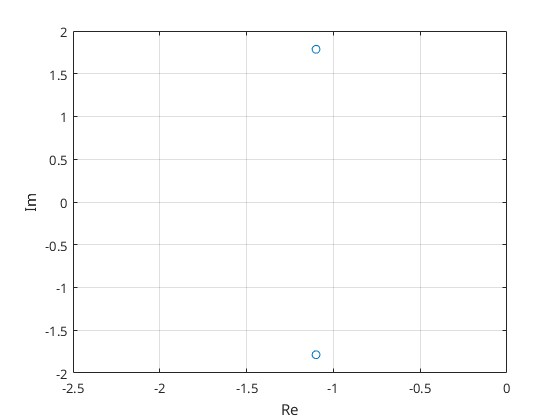
\includegraphics[width=0.65\textwidth]{poluses}
        \centering
        \caption{Полюсы передаточной функции}
        \label{fig:1}
    \end{figure} 
    \section{Найти изображение входного одиночного импульса воздействия и вычислить реакцию активной RC-цепи операторным методом; построить график реакции; приближенно оценить время затухания переходных процессов в цепи.}
    Найдем изображение импульса типа меандр (Рис. \ref{fig:2} )
    \begin{figure}[H]
        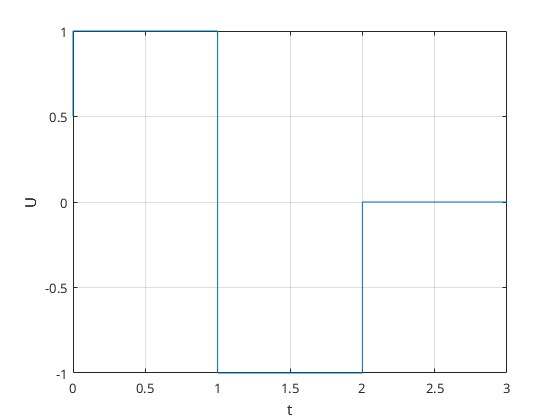
\includegraphics[width=0.65\textwidth]{imp}
        \centering
        \caption{Импульс меандр}
        \label{fig:2}
    \end{figure}
    С учетом данных таблицы \ref{1}, временная функция этого импульса будет выглядеть так:
    \begin{equation}
        u_1(t) = 3\delta (t) - 6\delta(t-1) + 3\delta(t-2),
    \end{equation}


    тогда изображение этого импульса:
    \begin{equation}
        U_1(S) = \frac{1}{S}\left(3e^{-2S} - 6e^{-S} + 3\right). 
    \end{equation}

    Расчитаем реакцию цепи операторным методом:
    \begin{multline}
        U_2(S) = H(S)\cdot U_1(S) =  \frac{5.52}{S^2 + 2.2S+ 4.4}
        \cdot \frac{1}{S}\left(3e^{-2S} - 6e^{-S} + 3\right) = \\
        = \frac{5.52\cdot3}{S(S^2 + 2.2S+ 4.4)}\cdot e^{-2S} -
        \frac{5.52\cdot6}{S(S^2 + 2.2S+ 4.4)}\cdot e^{-S} + \\
        + \frac{5.52\cdot3}{S(S^2 + 2.2S+ 4.4)}
    \end{multline}
    После разложения на простейшие и перехода {\it t}-область:
    \begin{multline}
        u_2(t) = 33.12\delta_1(1.0t - 1.0)
        (0.23e^{1.1 - 1.1t}(\cos(1.79t - 1.79) + \\
        + 0.62\sin(1.79t - 1.79)) - 0.23) - 
        3.76e^{-1.1t}(\cos(1.79t) + \\
        + 0.62\sin(1.79t)) - 16.56\delta_1(t - 2)(0.23e^{2.2 - 1.1t}
        (\cos(1.79t - 3.57) + \\
        + 0.62\sin(1.79t - 3.57)) - 
        0.23) + 3.76
    \end{multline}
    Построим график реакции:
    \begin{figure}[H]
        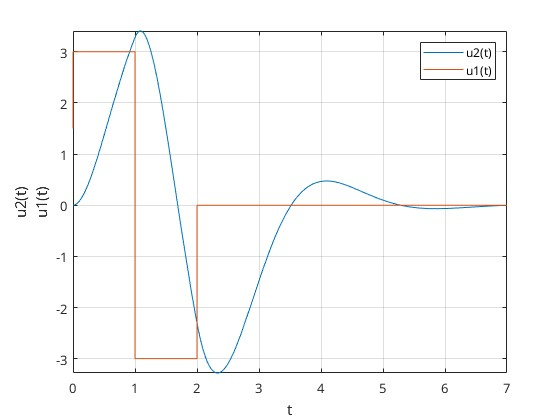
\includegraphics[width=0.8\textwidth]{react}
        \centering
        \caption{график реакции вместе с графиком воздействия}
    \end{figure}
    \section{Вычислить переходную и 
    импульсную характеристики активной цепи по
     заданной передаточной функции; построить их графики.}
    Вычислим переходную характеристику активной цепи:
    \begin{multline}
        H_1(S) = \frac{H(S)}{S}= \frac{5.52}{S(S^2 + 2.2S+ 4.4)} = 
        -\frac{0.63 + j0.39}{S+1.1 + j1.79} - \\ - \frac{0.63 - j0.39}{S + 1.1 - j1.79} + \frac{1.26}{S} 
    \end{multline}
    \begin{equation}
        h_1(t) = 1.26 - 1.26e^{-1.1t}(\cos(1.79t) + 0.62\sin(1.79t))
    \end{equation}
    Построим график переходной характеристики:
    \begin{figure}[H]
        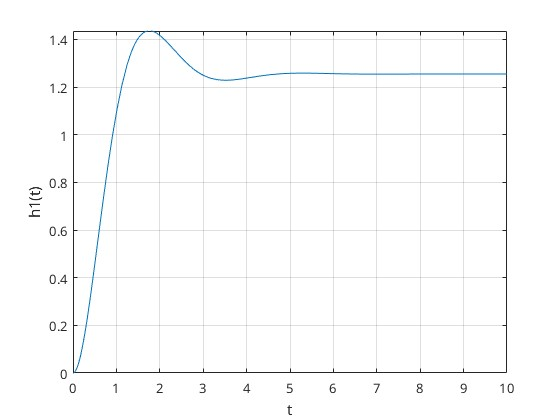
\includegraphics[width=0.8\textwidth]{h1}
        \centering
        \caption{Переходная характеристика}
    \end{figure}
    Вычислим импульсную характеристику активной цепи:
    \begin{multline}
        H(S) = \frac{5.52}{(S^2 + 2.2S+ 4.4)} = \frac{-1.54j}{S + 1.1 - j1.79} + \\ 
        + \frac{1.54j}{S - 1.1 + j1.79}
    \end{multline}
    \begin{equation}
        h(t) = 3.09e^{-1.1t}\sin(1.79t)
    \end{equation}
    Построим график импульсной характеристики:
    \begin{figure}[H]
        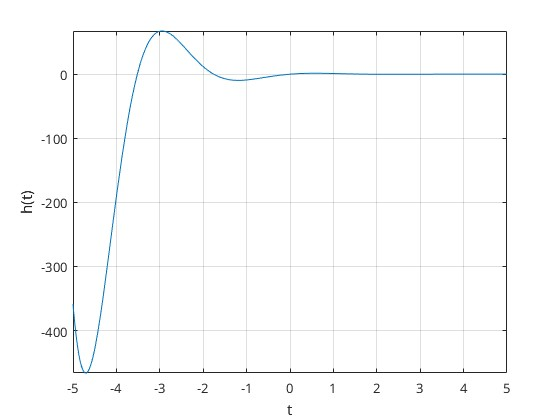
\includegraphics[width=0.8\textwidth]{h}
        \centering
        \caption{Импульсная характеристика}
    \end{figure}
    \section{Определить амплитудный и фазовый спектры входного одиночного импульса и построить их графики.}
    Входной одиночный импульс-меандр представлен на рисунке \ref{fig:1}.
    Определим амплитудный и фазовый спектры:
    \begin{multline}
        U_1(jw) = U_1(S)|_{jw} = \frac{1}{jw}\left(3e^{-2jw} - 6e^{-jw} + 3\right) = \\ 
         = \frac{3}{jw}e^{-jw}(e^{-jw} - 2 + e^{jw}) = 
         \frac{3}{jw}e^{-jw}\left(e^{-\frac{1}{2}jw} - e^{\frac12jw}\right)^2 = \\
         = j\frac{6}{w}e^{-jw}\sin^2\left(\frac12w\right)
    \end{multline} 
    \begin{equation}
        A(w) = \left| U_1(jw)\right| = 
        \frac{|j6e^{jw}\sin^2\left(\frac12w\right)
        |}{w} 
    \end{equation}
    \begin{multline*}
        A(w)|_{w=0}=\lim\limits_{w \to 0}
        \frac{|j6e^{jw}\sin^2\left(\frac12w\right)
        |}{w} = \lim\limits_{w \to 0}
        \frac{\left(6\sin^2\left(\frac12w\right)\right)'
        }{1} = \\
        = \lim\limits_{w \to 0}6\left(2sin\left(\frac12w\right)
        \frac12\cos\left(\frac12w\right)\right) = 0
    \end{multline*}
    \indent Значение спектрально плотности в нуле равно площади импульса, 
    что выполняется, т. к. алгебраическая площадь меандра равна нулю,\
    что видно из рис. \ref{fig:1}
    \begin{multline}
        \Phi(w) = \arg\left(
            j\frac{6}{w}e^{-jw}\sin^2\left(\frac12w\right)
            \right) = \\ = \arg\left(je^{-jw}\sin^2\left(\frac12w\right)\right) = 
            \frac{\pi}2 - w.
    \end{multline}
    \indent Построим графики амплитудной и фазовой спектральной плотности:
    \begin{figure}[H]
        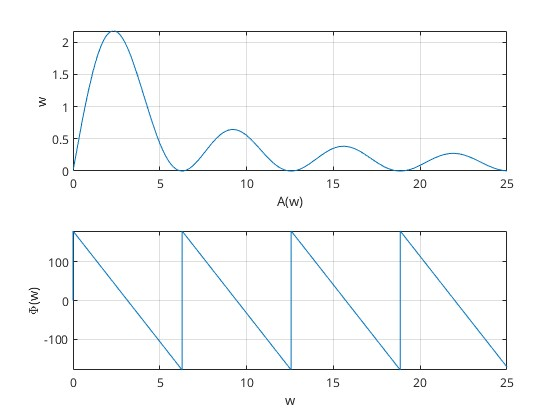
\includegraphics[width=0.8\textwidth]{awpw}
        \centering
        \caption{амплитудный и фазовый спектры одиночного импульса-меандра}
        \label{fig:6}
    \end{figure}
    \newpage
    \section{Определить амплитудный и фазовый спектры периодического 
    входного сигнала;
     ограничиться 10 гармониками разложения сигнала в ряд Фурье; 
     построить графики исходного входного периодического сигнала и сигнала, представленного рядом Фурье 
    (изобразить отдельно 3 первые составляющие ряда).}
    
\end{document}

